\documentclass[table,xcolor=dvipsnames,professionalfonts]{beamer}
\usepackage{xcolor}
\usepackage{booktabs}
\usepackage{graphicx}
\usepackage[percent]{overpic}
\usepackage{tikz}
\usepackage{feynmp}
\usepackage{xspace}
\usepackage{slashed}
%\usepackage[utopia]{mathdesign}
%\usepackage[charter]{mathdesign}
\usepackage[UKenglish]{babel}
\usepackage[utf8]{inputenc}
%\usepackage{lmodern}
\setbeamertemplate{navigation symbols}{}
\usepackage{appendixnumberbeamer}
%\usepackage{hepparticles}
%\usepackage{hepnicenames}
\usepackage{hepunits}
%\usepackage{bbm}

\ifpdf
\usepackage{epstopdf}
\usepackage[protrusion=true,expansion=true,tracking]{microtype}
%\DeclareGraphicsRule{*}{mps}{*}{}
\fi

\usepackage{listings}
\usepackage[framemethod=tikz]{mdframed}
\lstloadlanguages{C++}
\makeatletter
\newcommand{\srcsize}{\@setfontsize{\srcsize}{5pt}{5pt}}
\makeatother
\lstset{language=[11]C++,
  literate= % define some ligatures for PragmataPro
  {!!}{\texttt{!!}}2 {::}{\texttt{::}}2 {++}{\texttt{++}}2
  {--}{\texttt{--}}2 {()}{\texttt{()}}2 {\[\]}{\texttt{[]}}2
  {==}{\texttt{==}}2 {!=}{\texttt{!=}}2 {>=}{\texttt{>=}}2
  {<=}{\texttt{<=}}2 {&&}{\texttt{\&\&}}2 {||}{\texttt{||}}2
  {!>}{\texttt{!>}}2 {\#(}{\texttt{\#(}}2 {\#_}{\texttt{\#_}}2
  {\#\{}{\texttt{\#\{}}2 {\#?}{\texttt{\#?}}2 {\#>}{\texttt{\#>}}2
  {\%=}{\texttt{\%=}}2 {+=}{\texttt{+=}}2 {-=}{\texttt{-=}}2
  {*=}{\texttt{*=}}2 {/=}{\texttt{/=}}2 {&=}{\texttt{&=}}2
  {^=}{\texttt{^=}}2 {|=}{\texttt{|=}}2 {~=}{\texttt{~=}}2
  {<<}{\texttt{<<}}2 {>>}{\texttt{>>}}2 {->}{\texttt{->}}2
  {__}{\texttt{\_\_}}2
  {!!!}{\texttt{!!!}}3 {>>=}{\texttt{>>=}}3 {<<=}{\texttt{<<=}}3
  {/==}{\texttt{/==}}3 {...}{\texttt{...}}3,
  deletekeywords=[1]{auto,const,static,volatile,void,char,short,int,long,unsigned,float,double,inline,template,typename,namespace,class,union,struct,enum,true,false,nullptr},
  morekeywords=[2]{auto,const,static,volatile},
  morekeywords=[3]{void,char,short,int,long,unsigned,float,double,size_type,inline,iterator,const_iterator,reference,const_reference,Uninitialised,template,typename,namespace,class,union,struct,enum},
  morekeywords=[4]{std,our,LHCb,T,ARGS},
  morekeywords=[5]{true,false,nullptr,__LINE__,__FILE__,__func__},
  basicstyle=\srcsize\ttfamily\color{black},
  keywordstyle=[1]\color{magenta}\textbf,
  keywordstyle=[2]\color{orange}\textbf,
  keywordstyle=[3]\color{cyan}\textbf,
  keywordstyle=[4]\color{black},
  keywordstyle=[5]\color{violet!80!white},
  directivestyle=\color{blue!50!white},
  commentstyle=\color{blue}\textsl,
  stringstyle=\color{gray},
  identifierstyle=\color{green!50!black},
breaklines=true,breakautoindent=true}

\mdfdefinestyle{listing}{
  backgroundcolor=white!96!black,hidealllines,
  skipabove=0pt,skipbelow=0pt,
  leftmargin=0pt,rightmargin=0pt,
  innertopmargin=-5pt,innerbottommargin=-5pt,
  innerleftmargin=0pt,innerrightmargin=0pt,
  linewidth=0pt,middlelinewidth=0pt,
  startcode={\vspace{-3pt}},endcode={\vspace{-2ex}}
}
\surroundwithmdframed[style=listing]{lstlisting}

\usepackage{fontspec}
\setmainfont{Times New Roman}[]
%\setsansfont{FrontPagePro}[Scale=MatchLowercase]
%\IfFileExists{/usr/local/share/fonts/PragmataPro/PragmataPro_Mono_R_0826.ttf}{\setmonofont{PragmataPro}[Scale=MatchLowercase]}{}
%\setmonofont{Monoid.ttf}[Scale=MatchLowercase]
\setmonofont{Hack-Regular.ttf}[Scale=MatchLowercase]

\usetheme{Rochester}
%\usecolortheme{beaver}
\usecolortheme[named=NavyBlue]{structure}
\setbeamercolor{section in toc}{fg=black,bg=white}
%\setbeamercolor{alerted text}{fg=blue}
\setbeamercolor{structure}{fg=blue!80!black}
\setbeamercolor*{palette primary}{fg=black,bg=gray!30!white}
\setbeamercolor*{palette secondary}{fg=black,bg=gray!15!white}
\setbeamercolor*{palette tertiary}{bg=blue!80!black,fg=gray!10!white}
\setbeamercolor*{palette quaternary}{fg=blue,bg=gray!5!white}
\setbeamercolor*{sidebar}{fg=blue,bg=gray!15!white}
\setbeamercolor*{palette sidebar primary}{fg=blue!10!black}
\setbeamercolor*{palette sidebar secondary}{fg=white}
\setbeamercolor*{palette sidebar tertiary}{fg=blue!50!black}
\setbeamercolor*{palette sidebar quaternary}{fg=gray!10!white}
\setbeamercolor{titlelike}{parent=palette primary,fg=blue,bg=white}
\setbeamercolor{frametitle}{fg=white,bg=blue!80!black}
\setbeamercolor{frametitle right}{bg=gray!60!white}
\setbeamercolor*{separation line}{}
\setbeamercolor*{fine separation line}{}
\useinnertheme{rectangles}
\useoutertheme{infolines}
\usefonttheme[onlymath]{serif}
%\usefonttheme{professionalfonts}

%\loadgraphics{logo-pi-bunt3,lhcb-logo,unisiegel-gray}

% https://tex.stackexchange.com/a/98205
\newsavebox{\unilogo} \newsavebox{\pilogo} \newsavebox{\lhcblogo}
\IfFileExists{../cern-logo-gray.eps}{\sbox{\unilogo}{
\includegraphics[height=1.2cm]{../cern-logo-gray.eps}} }{\sbox{\unilogo}{
\includegraphics[height=1.2cm]{cern-logo-gray.eps}}}
\IfFileExists{../cern-logo.eps}{     \sbox{\pilogo}{
\includegraphics[height=0.75cm]{../cern-logo.eps}}      }{\sbox{\pilogo}{
\includegraphics[height=0.75cm]{cern-logo.eps}}     }
\IfFileExists{../lhcb-logo.eps}{\sbox{\lhcblogo}{
\includegraphics[height=0.75cm]{../lhcb-logo.eps}}}{\sbox{\lhcblogo}{
\includegraphics[height=0.75cm]{lhcb-logo.eps}}}

\setbeamertemplate{footline}
{
  \leavevmode%
  \hbox{%
    \begin{beamercolorbox}[wd=.333333\paperwidth,ht=2.25ex,dp=1ex,left]{author in head/foot}%
      \usebeamerfont{author in head/foot}\vtop{\vskip-2.25ex\hbox{\resizebox{!}{3.25ex}{\usebox{\pilogo}}}}%
      \hfill \insertshortauthor~~\insertshortinstitute \hfill%
    \end{beamercolorbox}%
    \begin{beamercolorbox}[wd=.333333\paperwidth,ht=2.25ex,dp=1ex,center]{title in head/foot}%
      \usebeamerfont{title in head/foot}\insertshorttitle%
    \end{beamercolorbox}%
    \begin{beamercolorbox}[wd=.333333\paperwidth,ht=2.25ex,dp=1ex,right]{date in head/foot}%
      \usebeamerfont{date in head/foot}\insertshortdate{}\hspace*{2em}%
      \insertframenumber{} / \inserttotalframenumber\hspace*{2ex} \vtop{\vskip-2.25ex\hbox{\resizebox{!}{3.25ex}{\usebox{\lhcblogo}}}}%
    \end{beamercolorbox}%
  }%
  \vskip0pt%
}

\setbeamertemplate{frametitle}
{
  \ifbeamercolorempty[bg]{frametitle}{}{\nointerlineskip}%
  \leavevmode%
  \vskip-2pt\hbox{%
    \begin{beamercolorbox}[wd=\paperwidth,left]{frametitle}%
      \usebeamerfont{frametitle}%
      \vskip.125ex%
      \hbox{\vtop{\raisebox{-1ex}[1ex][1ex]{\makebox[0pt][l]{\usebox{\unilogo}}}%
      \hspace{1em}\strut\insertframetitle\strut}\par%
      {%
        \ifx\insertframesubtitle\@empty%
        \else%
        {\usebeamerfont{framesubtitle}\usebeamercolor[fg]{framesubtitle}\insertframesubtitle\strut\par}%
        \fi
      }}%
    \end{beamercolorbox}%
  }%
}


\definecolor{bandgreen}{rgb}{0.3,0.8,0.2}
\newcommand{\FIXME}{{\color{red}FIXME}}
\newcommand{\arxiv}[1]{{\color{gray}\tiny$[$\href{http://arxiv.org/abs/#1}{arXiv:#1}$]$}}
\newcommand{\jref}[2]{{\color{gray}\tiny$[$\href{#2}{#1}$]$}}
\newcommand{\myhref}[2]{\href{#1}{\footnotesize{\textcolor{blue}{\texttt{#2}}}}}
\newcommand{\openref}[1]{\href{#1}{\footnotesize{\textcolor{blue}{\texttt{#1}}}}}


\author[~]{Lorenzo~Moneta~(CERN)\and
 %Markus~Stoye~(CERN)\and
 Michele~Floris~(University~of~Derby~and~CERN)\and
 Paul~Seyfert~(CERN)\and
 Sergei~Gleyzer~(University~of~Florida)\and
 Steven~Schramm~(Université~de~Genève)}
\institute[CERN]{}
\date[\today]{}
\title{IML meeting -- NEWS}


\begin{document}
\maketitle

\begin{frame}
  \frametitle{Announcements 1/2}

  \begin{itemize}
    \item Hadoop User forum
      \newline ``HEP Data Processing with Apache Spark''
      \newline Wednesday 6th Dec 2017, 14:00, at CERN
      \newline \openref{https://indico.cern.ch/event/678628/}
    \item Deep Learning for Physical Sciences workshop at NIPS
      \newline December 8, 2017, Long Beach (USA)
      \newline \openref{https://dl4physicalsciences.github.io/}
    \item next EP-IT data science seminar by  Conor Fitzpatrick (EPFL)
      \newline ``Too much of a good thing:\newline How to trigger in a signal-rich environment''
      \newline  Wednesday 13 Dec 2017, 11:00, at CERN
      \newline \openref{https://indico.cern.ch/event/675056/}
    \end{itemize}
  \end{frame}
  \begin{frame}
  \frametitle{Announcements 2/2}
    \begin{itemize}
    \item next IML meeting
      \newline Friday 26 Jan 2018, 222-R-001 (Filtration plant)
      \newline open topic, aiming for:
      \begin{itemize}
          \item followup on today's meeting
          \item news/summary from NIPS
          \item tools and software updates
          \item $<$your project here$>$
      \end{itemize}
      \openref{https://indico.cern.ch/event/679765/}
  \end{itemize}
\end{frame}

\begin{frame}
  \frametitle{2018 IML workshop}
  \begin{itemize}
      \item plans getting more and more concrete
        \newline ``core workshop'' 9th April -- 11th April
        \newline $\checkmark$ rooms booked
      \item similar to last time: physics sessions
        \newline topics: deep learning, tagging, regression, generative models
      \item new: hackathon 12th April (one day)
        \newline bring on your project (e.g.\ new feature for your favourite ML tool)
        \newline profit from expertise of the other participants around you
        \newline join and help others on their project
        \newline $\rightarrow$ suggest problems to attack at the hackathon
      \item different than last time: challenge
        \newline will start before the workshop (to run $\sim$ one month)
        \newline more details in 2018
  \end{itemize}
  \openref{https://indico.cern.ch/event/668017/}
\end{frame}

\begin{frame}
  \frametitle{today's topic: common benchmark dataset}
  \begin{columns}
    \begin{column}{.35\textwidth}
      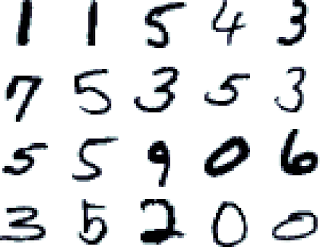
\includegraphics[width=\textwidth]{./mnist.png}
    \end{column}
    \begin{column}{.65\textwidth}
      what we want:
      \begin{itemize}
        \item ML benchmark(s)
        \item HEP specific
        \item common among experiments
        \item $\rightarrow$ able to compare two methods by looking up their benchmark
      \end{itemize}
    \end{column}
  \end{columns}
  \begin{block}{today's focus: technical challenges}
    \begin{itemize}
        \item make data accessible
        \item size, formats, \dots
        \item citing data
    \end{itemize}
  \end{block}
\end{frame}

\begin{frame}
  \frametitle{Agenda}
  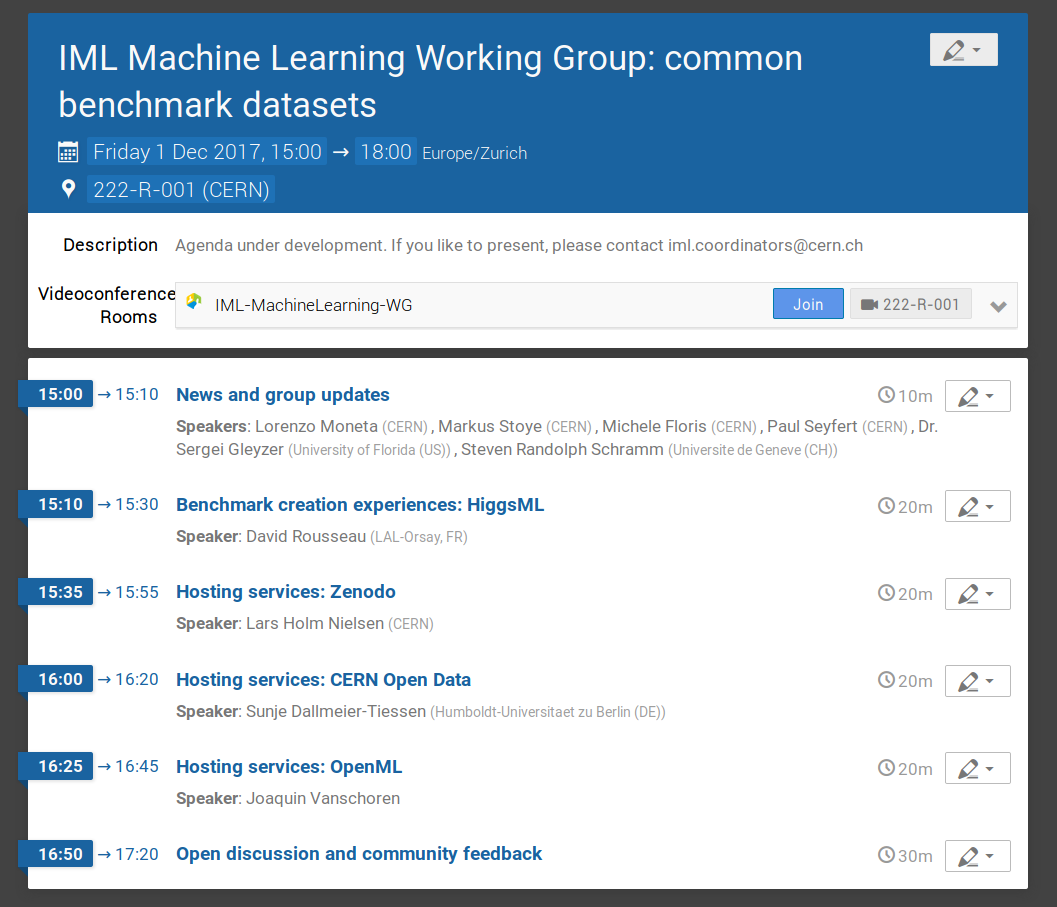
\includegraphics[width=.8\textwidth]{./agenda.png}
\end{frame}

\setbeamertemplate{background canvas}{%
  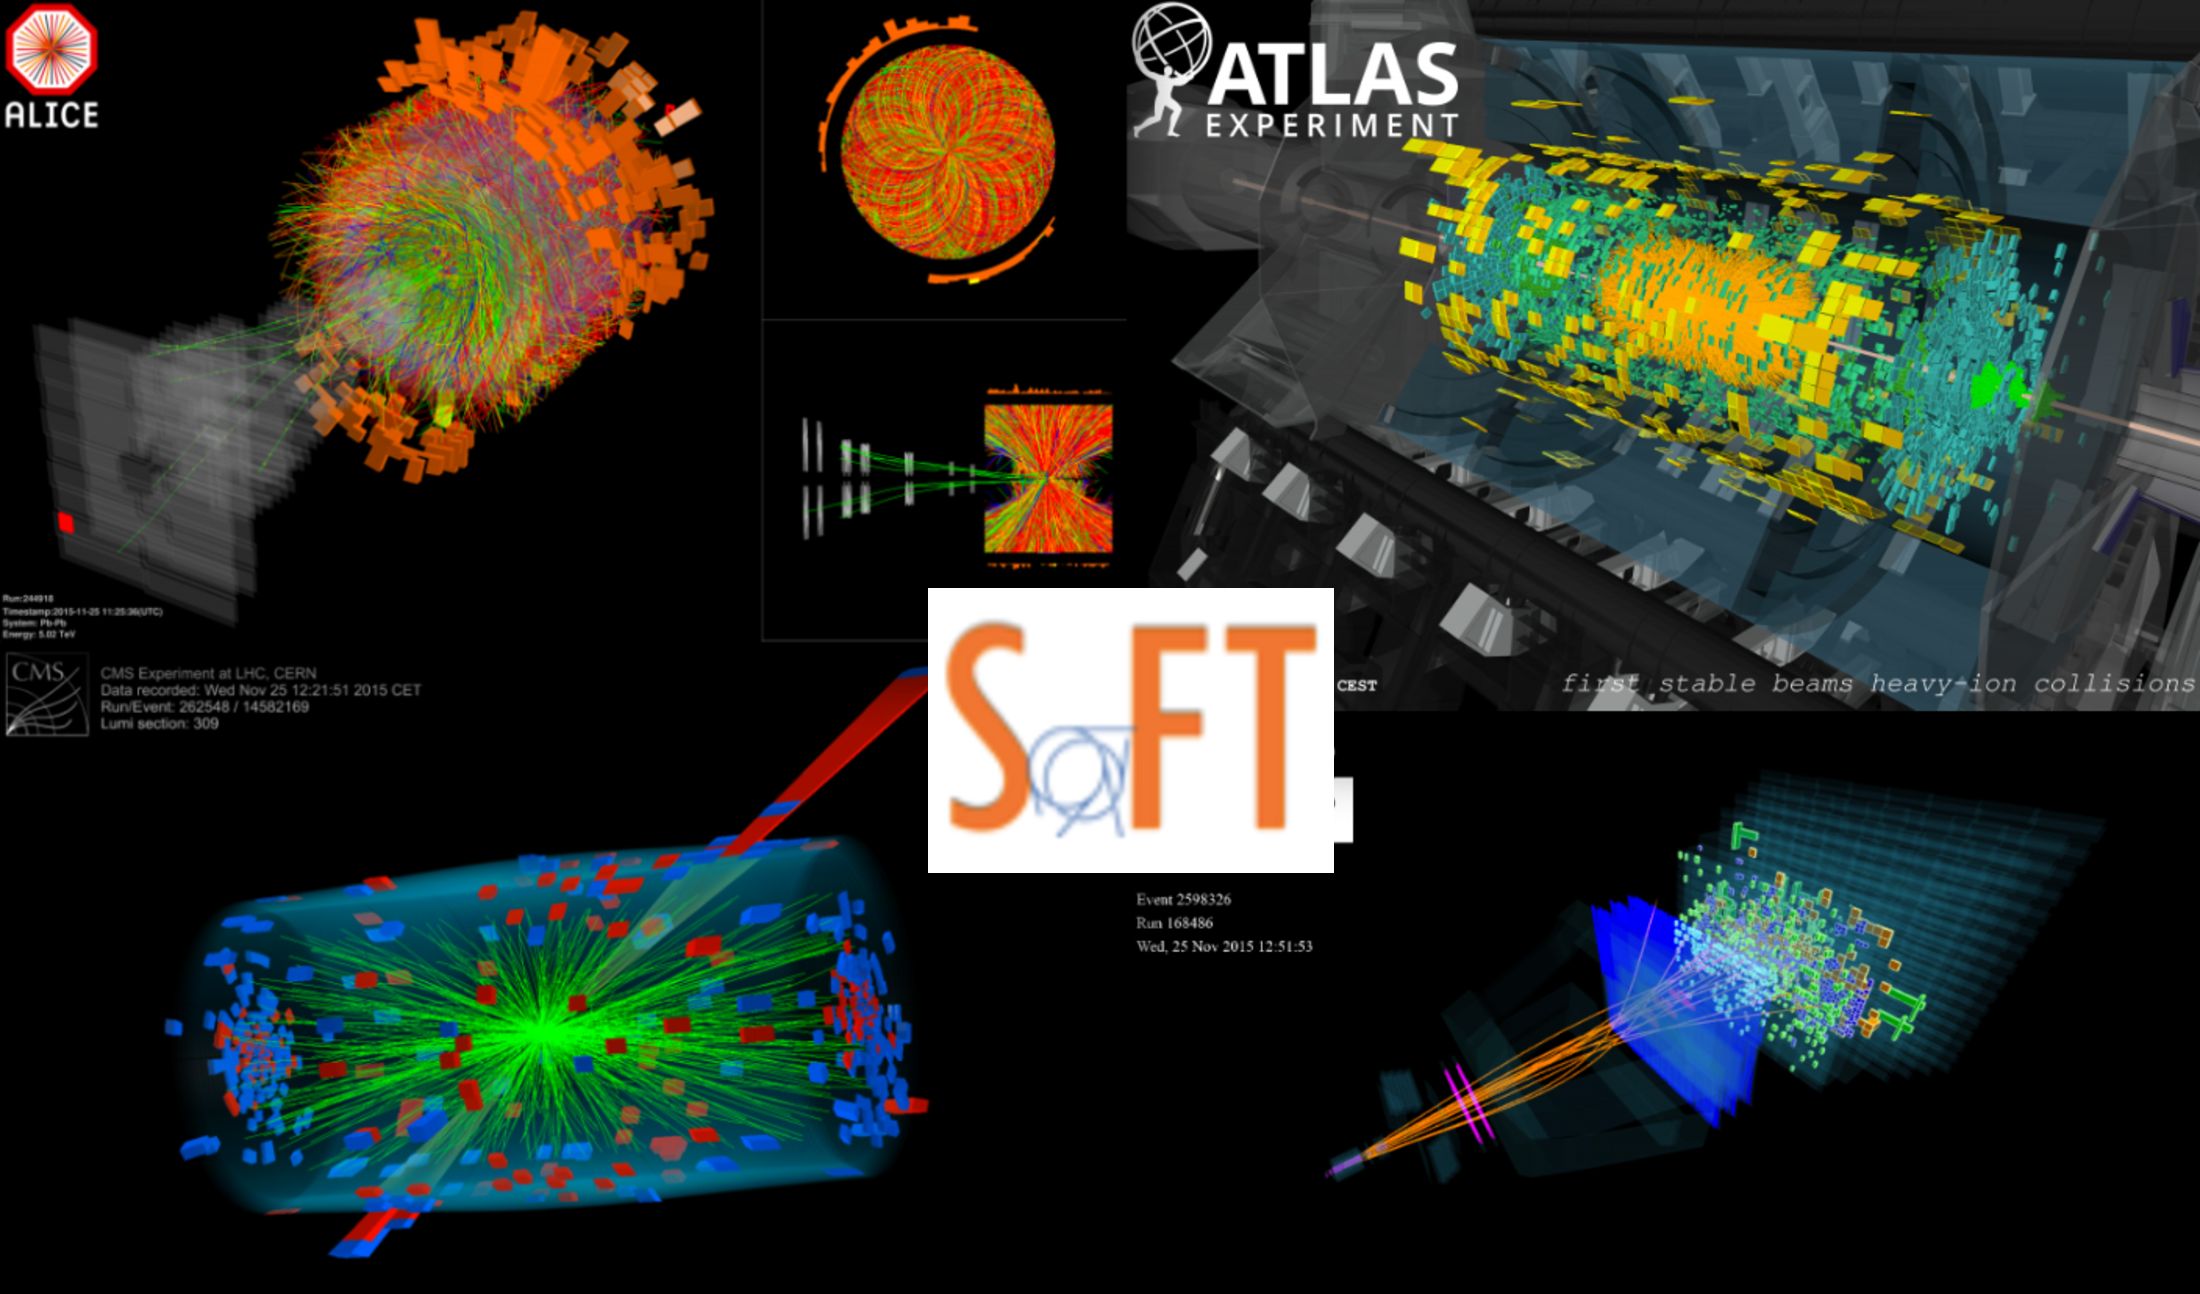
\includegraphics[width=\paperwidth,height=\paperheight]{banner.pdf}%
}   
\begin{frame}[t]
  \visible<2>{
    {~}
    \vspace{.5\textheight}
    \begin{columns}
      \begin{column}{.8\textwidth}
      \end{column}
      \begin{column}{.2\textwidth}
        \begin{block}{}
          \myhref{https://gitlab.cern.ch/pseyfert/slides-imlnews-2017-12-01}{sources for the slides}

          
\includegraphics[width=.9\textwidth]{./QR2.png}
        \end{block}
      \end{column}
      \end{columns}
    }
\end{frame}
  \beamertemplateshadingbackground{Black!03}{White}


\appendix

%\begin{frame}
%  \frametitle{BACKUP}
%  backup is for people who can't improvise
%
%  (yes, that's a cheap excuse for not preparing backup slides)
%\end{frame}

\end{document}
